\section{Question 8}
\subsection{Part a}
We use Proposition 4.8 from Koller-Friedman: Let G be any Bayesian network graph. The moralized graph M[G] is a minimal I-map for G.\\
That gives us the following diagram equivalent Markov network.\\
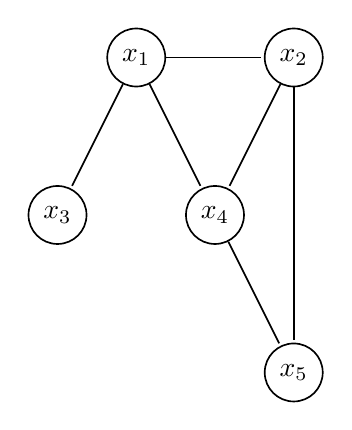
\begin{tikzpicture}[
    > = stealth, % arrow head style
    shorten > = 1pt, % space from node to arrow
    auto,
    node distance = 2cm, % distance between nodes
    semithick % line style
]

% Nodes
\node[draw, circle] (x1) at (0, 2) {$x_1$};
\node[draw, circle] (x2) at (2, 2) {$x_2$};
\node[draw, circle] (x3) at (-1, 0) {$x_3$};
\node[draw, circle] (x4) at (1, 0) {$x_4$};
\node[draw, circle] (x5) at (2, -2) {$x_5$};

% Edges
\draw[-] (x1) -- (x2);
\draw[-] (x1) -- (x3);
\draw[-] (x1) -- (x4);
\draw[-] (x2) -- (x4);
\draw[-] (x2) -- (x5);
\draw[-] (x4) -- (x5);

\end{tikzpicture}

\subsection{Part b}
$x_1 \independent x_2$ and $x_1 \independent x_2 | x_3$ are two CIs that hold in G but not in H.